\documentclass{article}
\usepackage[margin=3cm]{geometry}
\usepackage[utf8]{inputenc}
\usepackage{amsmath}
\usepackage{amssymb}
\usepackage{float}
\usepackage{enumitem}
\usepackage{graphicx}
\usepackage{caption}
\usepackage{subcaption}
\usepackage{eurosym}

\usepackage{comment}

\graphicspath{ {Plots/} }


\begin{document}
	\textit{MS-E2134 - Decision making and problem solving}
	\vfill
	{\centering \Huge Assignment 3 \par}
	\vfill
	Christian Segercrantz - 481056 \\
	\par \today
	\pagebreak
	\tableofcontents
	\pagebreak
\section{Attribute-specific value functions - value functions}
The value functions are as follows:
\begin{align}
	v_1(x_1) =& \frac{1}{40}x_1 \\
	v_2(x_2) =& 
		\begin{cases}
		 0,& 0 \leq x_2 \leq 2 \\
		 \frac{1}{12}x_2 -\frac{1}{6},& 2 \leq x_2 < 6 \\
		 \frac{1}{27}x_2 +\frac{1}{9},& 6 \leq x_2 < 15 \\
		 \frac{1}{45}x_2 +\frac{1}{3},& 15 \leq x_2 \leq 30
		\end{cases}\\
	v_3(x_3) =&
		\begin{cases}
			\frac{1}{14}x_3 - \frac{1}{7} & 2 \leq x <9\\
			\frac{1}{42}x_3 + \frac{2}{7} & 9 \leq x \leq 30
		\end{cases} \\
	v_4(x_4) =& \frac{1}{18}x_4 - \frac{1}{9}\\ 
	v_5(x_5) =& \frac{1}{20}x_5\\
	v_6(x_6) =& \frac{1}{20}x_6\\
	v_7(x_7) =& \frac{1}{100}x_7\\
	v_8(x_8) =& 
		\begin{cases}
			\frac{1024}{1023}\left(1-2^{-x_8}\right) & 0 \leq x_8 < 10 \\
			1 &  10 \leq x_8
		\end{cases} \\
	v_9(x_9) =&
		\begin{cases}
			 \frac{1}{4}(1-\sqrt{5})\left(1-\left(\frac{1}{2}\left(1+\sqrt{5}\right)\right)^{3-x_9}\right) & 0 \leq x_9 < 3 \\
			 0 & 3 \leq x_9
		\end{cases}
\end{align}
For the derivation for $v_1, v_2, v_3, v_4, v_5, v_6, v_7$ simple linear interpolation was used based on the given facts. The derivation for $v_9$ can be seen below.
%\begin{comment} v_9 derivation
\begin{equation}
B+A(1-e^{-(3-x_9)/r}) \text{ and } v_9(0)-v_9(1) = v_9(1) - v_9(3)
\end{equation}

\begin{align}
&B+A(1-e^{-(3-x_9)/r})\\ 
v_9(3) = 0 =& B+A(1-e^{-(3-3)/r}) \iff B= 0 \\
v_9(0) = 1 =& A(1-e^{-(3-0)/r}) \\
& \frac{1}{A}= 1 - e^{-3/r} \\
& A= \frac{1}{1-u^3} \\
\end{align}
\begin{align}
v_9(100)= 0 =& A(1-e^{-(3-100)/r})\\
\end{align}
\begin{align}
v_9(0)-v_9(1) &= v_9(1) - v_9(3)\\
2v_9(1) &= v_9(0)\\
v_9(1) &= \frac{1}{2}\\
\frac{1}{2} &= \frac{1}{1-u^3}(1-u^{2})\\
1-u^3 &= 2-2u^2\\
-u^3 + 2u^2 - 1 &= 0 \implies  u=\frac{1}{2}+\frac{\sqrt{5}}{2} \left(\lor u=1 \lor u=\frac{1}{2}-\frac{\sqrt{5}}{2}\right) \\
e^{-1/r} &= 	\frac{1}{2}+\frac{\sqrt{5}}{2} \iff r = \frac{1}{ln(2) - ln(1 + sqrt(5))}	\\
\implies A&= \frac{1}{1-( 1/2 + sqrt(5)/2)} \iff A= \frac{1}{4}(1-\sqrt{5}) \\
\implies v_9&= \frac{1}{4}(1-\sqrt{5})\left(1-\left(\frac{1}{2}\left(1+\sqrt{5}\right)^{(3-x_9)}\right)\right)
\end{align}
%\end{comment}
\section{Attribute-specific value functions - values}
		The attribute values for all alternatives can be found from the attached excel.
\section{Attribute-specific value functions - value plots}
	\begin{figure}[H]
		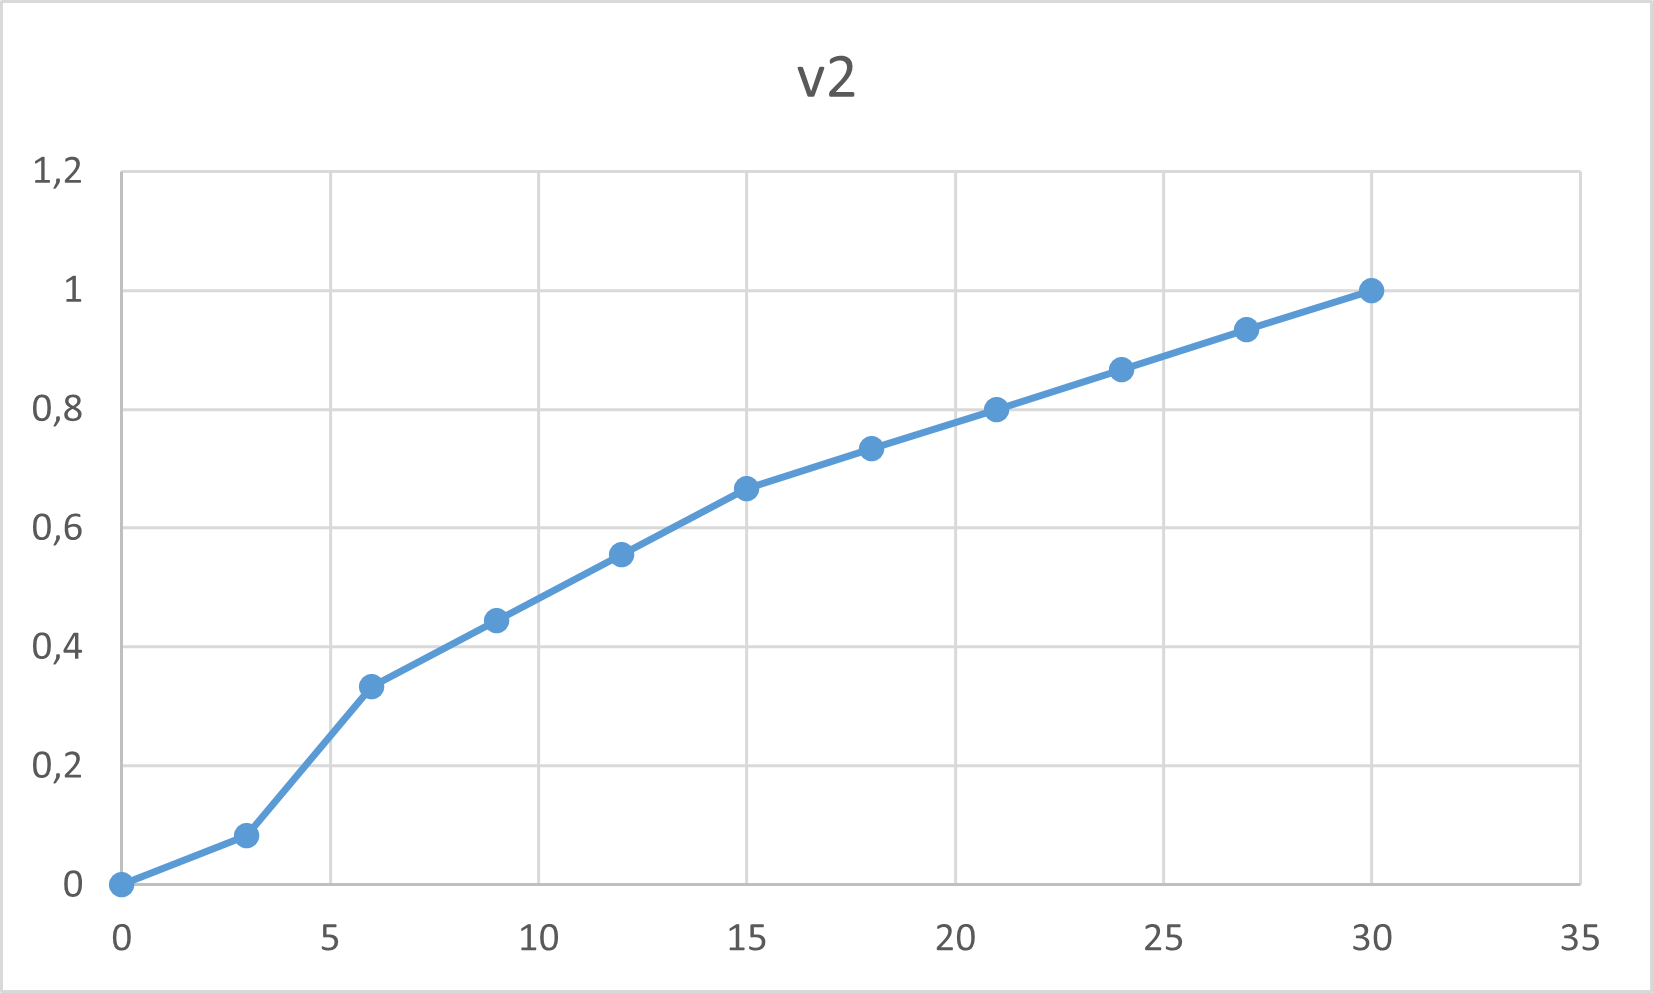
\includegraphics[width=0.8\textwidth]{3_v2.png}
		\caption{The plot for $v_2$.}
		\label{fig:3_v2}
	\end{figure}
	\begin{figure}[H]
		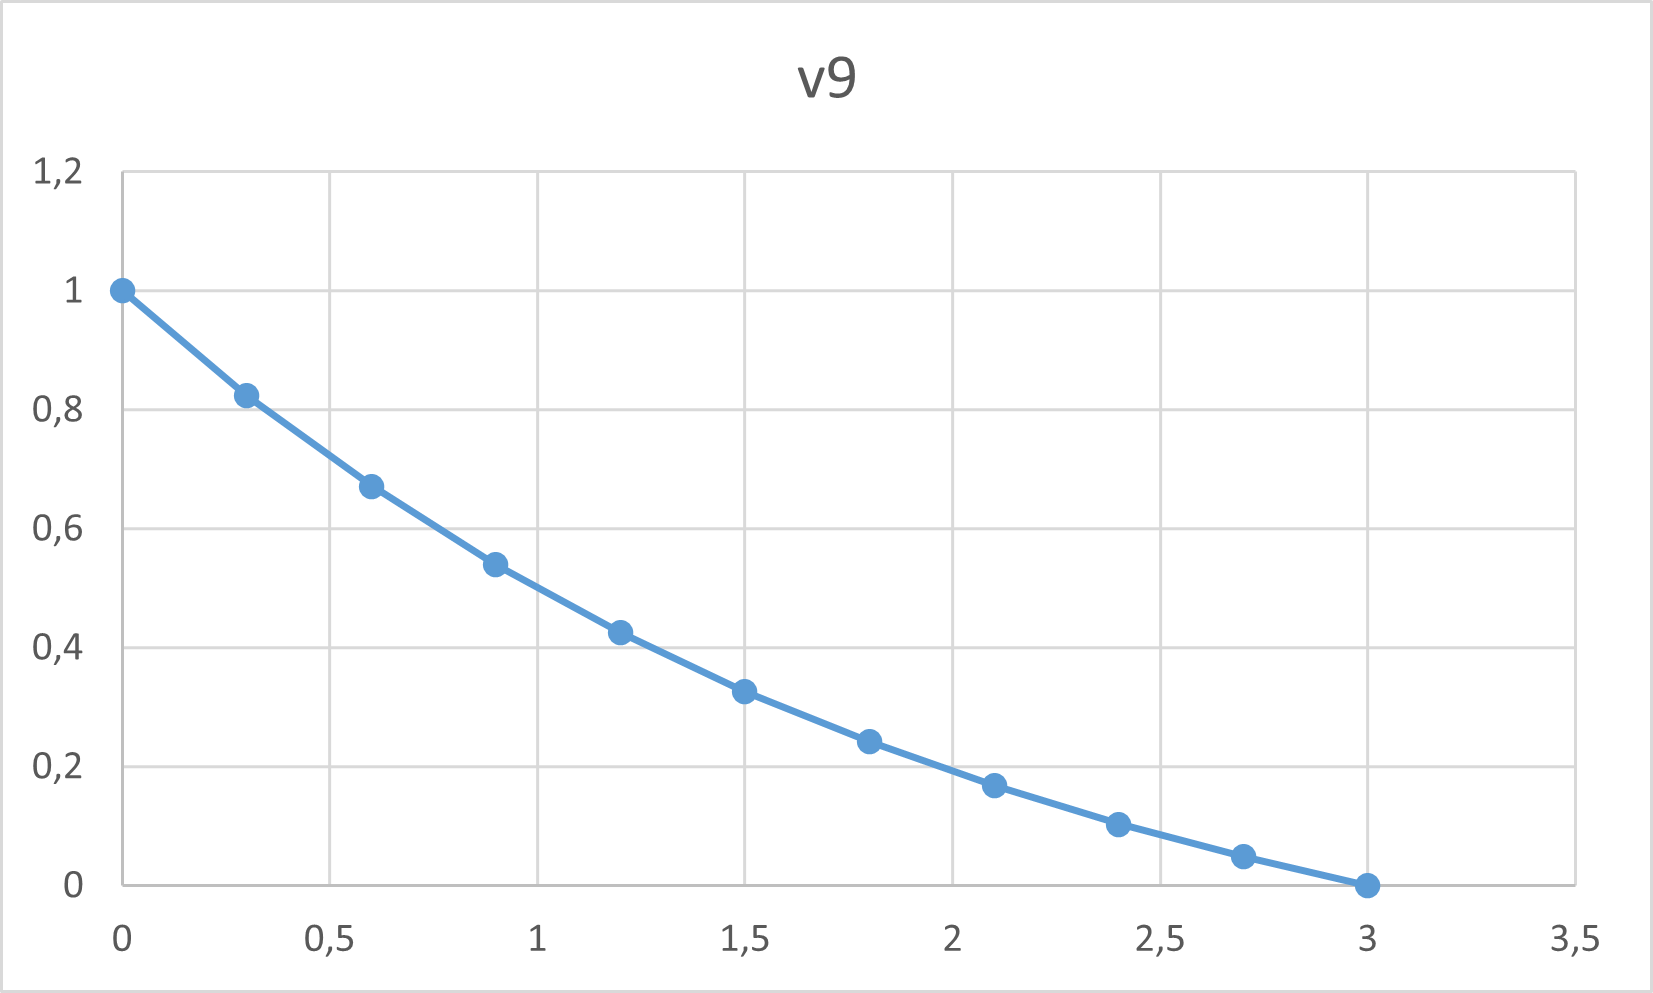
\includegraphics[width=0.8\textwidth]{3_v9.png}
		\caption{The plot for $v_9$.}
		\label{fig:3_v9}
	\end{figure}
\section{Attribute weights}
	From 1. , and knowing that 20 is the max and 0 the min for both value functions, we get the equation
	\begin{align}
		\frac{w_5 v_5(20)-w_5 v_5(0)}{w_6v_6(20)-w_6v_6(0)} &= \frac{40}{45}\\
		w_5 = \frac{8}{9}w_6.
	\end{align}
	From 2., and knowing that the max value is 20 and min value is 2, we get
	\begin{align}
		\frac{w_6 v_6(20)-w_6 v_6(0)}{w_4v_4(20)-w_4v_4(2)} &= \frac{45}{30}.\\
		w_4 = \frac{2}{3}w_6.
	\end{align}
	From 3. we get information about two equally preferred preferences, and again remembering the min value of the value functions,
	\begin{align}
		w_8v_8(1) - w_8v_8(0) &= w_4v_4(10) - w_4v_4(2)\\
		w_8 &=  \frac{v_4(10)}{v_8(1)}w_4.
	\end{align}
	From 4. we get a similar equation as above
	\begin{align}
		w_7v_7(1) - w_7v_7(0) &= w_4v_4(3) - w_4v_4(2)\\
		w_7 &=  \frac{v_4(3)}{v_7(1)}w_4.
	\end{align}
	From 5.	get multiple the following equality
	\begin{align}
		w_1v_1(40) - w_1v_1(0) &= w_2v_2(30) - w_2v_2(0) + w_3v_3(20) - w_3v_3(0)\\
		w_1 &= w_2 + w_3v_3(20).
	\end{align}
	In 6., we know that all but two values do not change, hence we can omit them from the start
	\begin{align}
		w_1v_1(40) + w_9v_9(1.2) &= w_1v_1(10) + w_9v_9(0)\\
		w_1 + w_9v_9(1.2) &= w_1v_1(10) + w_9\\
		w_1(1-v_1(10))&=w_9(1-v_9(1.2))\\
		w_9&=\frac{1-v_1(10)}{1-v_9(1.2)}w_1.
	\end{align}
	In 7., we know that the two changes from the minimum $x^0$ are equally preferred, i.e
	\begin{align}
		w_4v_4(10) + w_9v_9(1.2) - w_4v_4(2) - w_9v_9(100) &= w_4v_4(18) + w_9v_9(3) - w_4v_4(2) - w_9v_9(100)\\
		w_4v_4(10) + w_9v_9(1.2) &= w_4v_4(18) + w_9v_9(3)\\
		w_4v_4(10) + w_9v_9(1.2) &= w_4v_4(18)\\
		w_9 = \frac{v_4(18)-v_4(10)}{v_9(1.2)}w_4.
	\end{align}
	From 8. we get
	\begin{align}
		w_2v_2(15)-w_2v_2(0) &= w_3v_3(30)-w_3v_3(2)\\
		w_2v_2(15) &= w_3.
	\end{align}
	Additionally we know that the sum of weights equals to one 
	\begin{equation}
		\sum_{i=1}^{9}w_i=1.
	\end{equation}
	By solving these equations, we get the following values
	\begin{alignat}{3}
		w_1&= 0.062131...& \approx 0.06,\\
		w_2&= 0.0412027...&\approx0.04,\\
		w_3&= 0.0274685...&\approx0.03,\\
		w_4&= 0.076779...&\approx0.08,\\
		w_5&= 0.102372...&\approx0.10,\\
		w_6&= 0.115168..&\approx0.12,\\
		w_7&= 0.42655...&\approx0.43,\\
		w_8&= 0.0681814...&\approx0.07,\\
		w_9&= 0.080147...&\approx0.08.
	\end{alignat}
\section{Overall values}
	Table \ref{tab:ex5} displays the normalized values of the sites times the area.
	\begin{table}[H]
		\centering
		\caption{Normalized vlaue functions of the sites times the area.}
		\label{tab:ex5}
		\begin{tabular}{lll}
			\textbf{Site} & \textbf{Area} & \textbf{Normalizied value} \\ \hline
			1             & 1,2           & 0,26                       \\
			2             & 3             & 0,88                       \\
			3             & 2,1           & 0,71                       \\
			4             & 3             & 0,64                       \\
			5             & 0,8           & 0,25                       \\
			6             & 2             & 0,70                       \\
			7             & 3             & 0,70                       \\
			8             & 0,9           & 0,23                       \\
			9             & 1,1           & 0,37                       \\
			10            & 2,4           & 0,48                      
		\end{tabular}
	\end{table}
\section{Recalculated overall values}
	Since $a_7$ most preferred level changes from 100 to 40, the value function  becomes $v_7=\frac{1}{40}x_7$. Thus, the only value in our system of equations for solving the weights that change is $v_7(1)$. The recalculated weights are
	\begin{alignat}{3}
		w_1&= 0.0835016...& \approx 0.08,\\
		w_2&= 0.0553747...&\approx0.06,\\
		w_3&= 0.0369165...&\approx0.04,\\
		w_4&= 0.103188...&\approx0.10,\\
		w_5&= 0.137584...&\approx0.14,\\
		w_6&= 0.154782..&\approx0.15,\\
		w_7&= 0.229306...&\approx0.23,\\
		w_8&= 0.091633...&\approx0.09,\\
		w_9&= 0.107714...&\approx0.11.
	\end{alignat}
	and the scores can be sen in Table \ref{tab:ex6}.
	\begin{table}[]
		\centering
		\caption{Normalized value functions of the sites times the area.}
		\label{tab:ex6}
		\begin{tabular}{lll}
			\textbf{Site} & \textbf{Area} & \textbf{Normalizied value} \\ \hline
			1             & 1,2           & 0,34                       \\
			2             & 3             & 1,18                       \\
			3             & 2,1           & 0,95                       \\
			4             & 3             & 0,86                       \\
			5             & 0,8           & 0,34                       \\
			6             & 2             & 0,94                       \\
			7             & 3             & 0,94                       \\
			8             & 0,9           & 0,31                       \\
			9             & 1,1           & 0,50                       \\
			10            & 2,4           & 0,65                      
		\end{tabular}
	\end{table}

	If we calculate $\frac{V_i'(x_i)}{V_i(x_i)}$ we get a constant $\alpha\approx1.34$ for all $i$. This suggest that $V_i'(x_i)=\alpha V_i(x_i)$ for all $i$, i.e. the $V'$ is a affine transformation of $V$. 
	
\section{Site combination selection}
	The binary linear optimization problem we need to solve is
	\begin{alignat}{3}
		\max_y& \sum_{j=1}^{10} V(x^j)y_j\\
		\text{subject to} & \sum_{j=1}^{10} c_jy_j &\leq 25000\\
		&y_j \in \mathbb{B},
	\end{alignat}
	where b is a binary variable indicating if a site is to be acquired. 
	
	The calculations for this part is done in the attached excel. The optimal solution are the following sites: 2, 3, 5, 6, 7, 9. This gives a optimal value of approximately $4,85$ at a cost of 24494\euro.

\section{Multi-objective optimization applied to site combination selection - optimization}
The figure produced by the script can be seen in Figure \ref{fig:8_first_run}.
	\begin{figure}[H]
		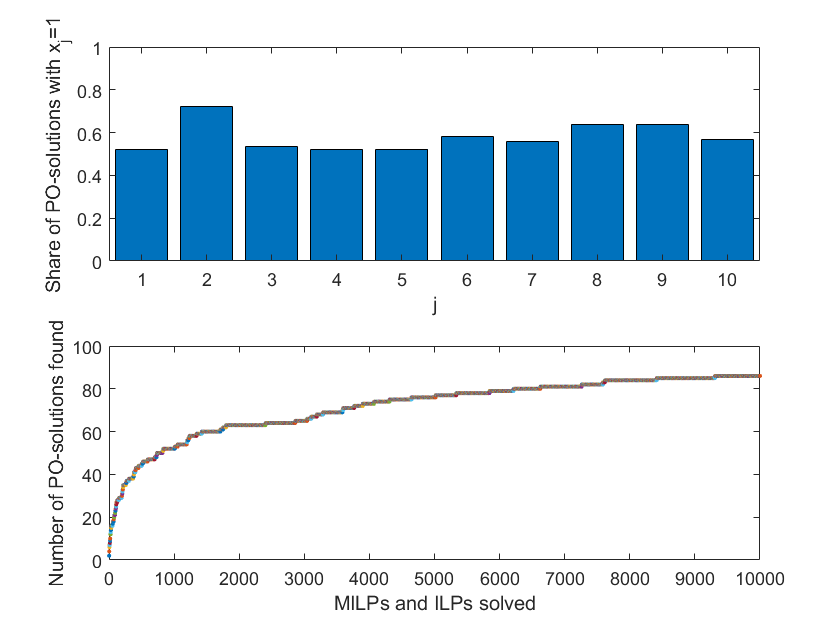
\includegraphics[width=0.8\textwidth]{8_first_run.png}
		\caption{The pareto optimal solutions and core indexes.}
		\label{fig:8_first_run}
	\end{figure}
	  

\section{Multi-objective optimization applied to site combination selection - solutions}
86 different pareto optimal solutions were found by the algorithm. The solution is among them, the 7th found pareto optimal solution. The results do not change significantly by running the script multiple times, all pareto optimal solutions aren't found each time. The core indices are roughly the same however.

\section{Multi-objective optimization applied to site combination selection - core indices}
The site with the highest core index is site 2 with an approximately index of $72\%$ and the lowest core index are sites 1,4,	 and 5 with approximately $52\%$.

\section{Robustness analysis of site combination selection - Formulation of feasibility region}
The feasible region of $S$ can be defined as 
\begin{align}
	S &= \{w_i:i=1...9|0.8r_i\leq \frac{w_i}{w_7} \leq 1.25r_i \forall i,\sum_{i=1}^{9} w_i = 1\}\\
	r_i &= \frac{w_i^*}{w_7^*}\\	
\end{align}
From here we can formulate the linear constraint as 
\begin{align}
	0.8\frac{w_i^*}{w_7^*}w_7 - w_i &\leq 0 \qquad \forall i \\
	w_i - 1.25\frac{w_i^*}{w_7^*}w_7 &\leq 0 \qquad \forall i
\end{align}
\section{Robustness analysis of site combination selection - Tables}
Table \ref{tab:aw} shows the matrix $A_w$ and $B_w$ is simply a $18\times 1$ vector full of zeros.
\begin{table}[H]
	\centering
	\caption{$A_w$}
	\label{tab:aw}
	\begin{tabular}{lllllllll}
		-1 & 0  & 0  & 0  & 0  & 0  & 0.291319372367055  & 0  & 0  \\
		0  & -1 & 0  & 0  & 0  & 0  & 0.193190583761437  & 0  & 0  \\
		0  & 0  & -1 & 0  & 0  & 0  & 0.128793838800555  & 0  & 0  \\
		0  & 0  & 0  & -1 & 0  & 0  & 0.360001046636372  & 0  & 0  \\
		0  & 0  & 0  & 0  & -1 & 0  & 0.480001395515163  & 0  & 0  \\
		0  & 0  & 0  & 0  & 0  & -1 & 0.540001569954559  & 0  & 0  \\
		0  & 0  & 0  & 0  & 0  & 0  & -0.200000000000000 & 0  & 0  \\
		0  & 0  & 0  & 0  & 0  & 0  & 0.319688102361037  & -1 & 0  \\
		0  & 0  & 0  & 0  & 0  & 0  & 0.375791300707352  & 0  & -1 \\
		1  & 0  & 0  & 0  & 0  & 0  & -0.455186519323524 & 0  & 0  \\
		0  & 1  & 0  & 0  & 0  & 0  & -0.301860287127245 & 0  & 0  \\
		0  & 0  & 1  & 0  & 0  & 0  & -0.201240373125867 & 0  & 0  \\
		0  & 0  & 0  & 1  & 0  & 0  & -0.562501635369332 & 0  & 0  \\
		0  & 0  & 0  & 0  & 1  & 0  & -0.750002180492442 & 0  & 0  \\
		0  & 0  & 0  & 0  & 0  & 1  & -0.843752453053998 & 0  & 0  \\
		0  & 0  & 0  & 0  & 0  & 0  & -0.250000000000000 & 0  & 0  \\
		0  & 0  & 0  & 0  & 0  & 0  & -0.499512659939121 & 1  & 0  \\
		0  & 0  & 0  & 0  & 0  & 0  & -0.587173907355237 & 0  & 1 
	\end{tabular}
\end{table}
\section{Robustness analysis of site combination selection - Feasible site combinations}
We get the number of feasible site combinations as the non-zero values of the vector F: 736.

\section{Robustness analysis of site combination selection - Non-dominated feasible combinations}
The number of non-dominated, and feasible according to our linear constraints, solutions can be seen from $Z_{ND}$ and is 3.
\section{Robustness analysis of site combination selection - Non-dominated sites}
The sites that are non-dominated and feasible according to our linear constraints are 2, 3, 6, and 9. 
\section{Robustness analysis of site combination selection - Previous solution}
The reason our previous solution is found among the non-dominated ones is that our original weights are within the feasible region and a optimal solution is always a non-dominated solution. 
\section{Robustness analysis of site combination selection - Non-dominated combinations}
The number of non-dominated solutions can be seen from $Z_{ND2}$ and is 82.
\section{Robustness analysis of site combination selection - }
Since the amount of solutions found in part 8 is larger than in 17, we can for sure conclude that there are not in the set of non-dominated solutions. This can happen 

\section{Robustness analysis of site combination selection - }
We can find 37 solutions that are non-dominated but not optimal. This is since a solution can be non-dominated without being optimal. We have clear examples of this in the lecture slides, for example slide 6b slide 22. 
\end{document}